\documentclass[12pt]{article}
\usepackage{geometry}
\usepackage{graphicx}
\usepackage{amsmath} 
\usepackage{hyperref}
\usepackage{cleveref}
\usepackage{setspace}
\usepackage{fancyhdr} % For custom headers and footers

% Set tighter page margins
\geometry{top=0.75in, bottom=0.75in, left=0.75in, right=0.75in}

% Reduce line spacing
\setstretch{0.9}

% Customize header and footer
\pagestyle{fancy}
\fancyhf{} % Clear all headers and footers

% Add custom header
\fancyhead[L]{\textbf{Distributed Systems (CS60064)}} % Left-aligned subject name and number

% Add custom footer
\fancyfoot[L]{\textbf{Bratin Mondal}} % Left-aligned student name
\fancyfoot[R]{\textbf{Roll No: 21CS10016}} % Right-aligned roll number
\fancyfoot[C]{\thepage} % Center-aligned page number

\sloppy

\begin{document}

% Header for the first page
\begin{center}
    \textbf{\huge Assignment 1} \\[1em]
    \textbf{Student Name:} Bratin Mondal \\[0.5em]
    \textbf{Roll Number:} 21CS10016 \\[0.5em]
    \textbf{Course Name:} Distributed Systems \\[0.5em]
    \textbf{Course Number:} CS60064
\end{center}

% Include Problem 1
\section{Problem 1}\label{prob1}
Let us assume that the client sent the query message at \( t = 0 \). The message took \( x \) milliseconds to reach the server. Since nothing has been specified regarding the server's processing time, we assume it is negligible. The server sends the response message at \( t = x \), and the response message took \( y \) milliseconds to reach the client. The client receives the response message at \( t = x + y \). The client then takes 1 millisecond to process the message and finally sets its clock to the server's clock at \( t = x + y + 1 \). It is given that \( x \leq 2 \) and \( y \leq 2 \). (Here, all time values are with respect to a global reference time.)

% Include a figure
\begin{figure}[h]
    \centering
    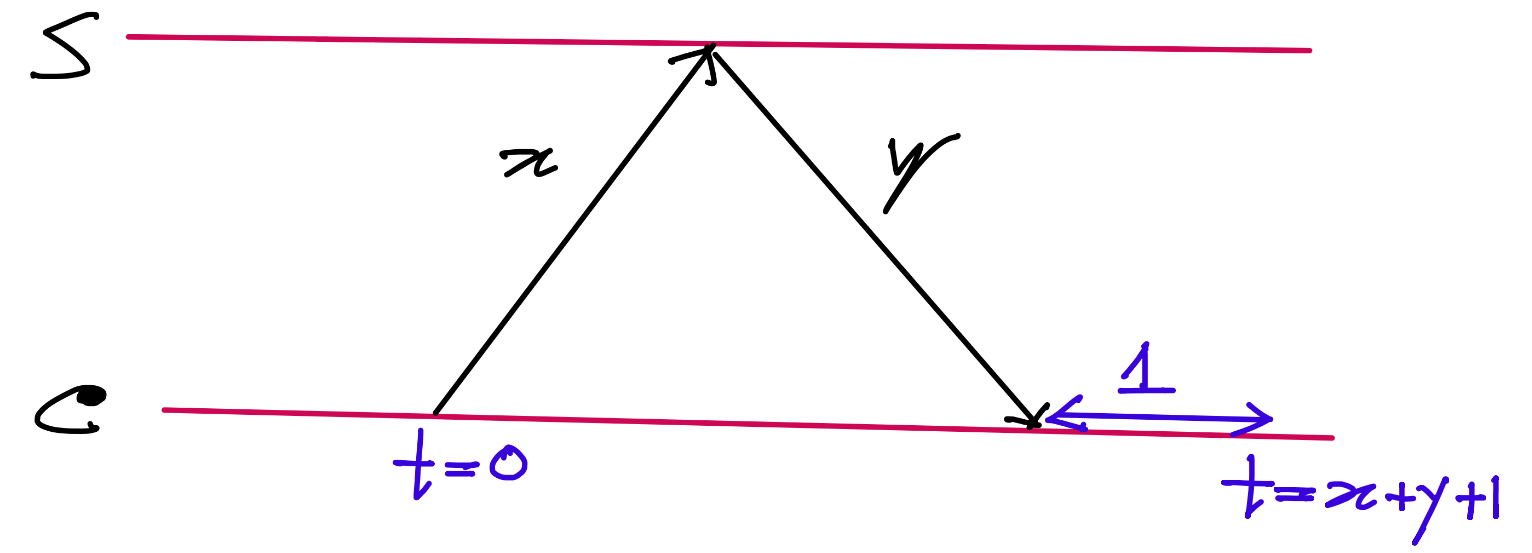
\includegraphics[width=0.5\textwidth]{IMG/Q1.jpeg}
    \caption{Timeline of Client-Server Communication}
    \label{fig:example}
\end{figure}

The server receives the query message at \( t = x \) and immediately sends the response message. The response message to the client contains only this value. Now, the client estimates the round-trip time (RTT) as:
\[
\text{RTT} = x + y + 1
\]
The client adds \( \frac{\text{RTT}}{2} \) to its clock to synchronize with the server's clock. Therefore, at \( t = x + y + 1 \), the client's clock is set to:
\[
\text{Client's Clock} = x + \frac{x + y + 1}{2}
\]
Meanwhile, the server's clock has the correct value:
\[
\text{Server's Clock} = x + y + 1
\]

The difference between the server's clock and the client's clock is given by:
\[
\text{Server's Clock} - \text{Client's Clock} = \frac{y + 1 - x}{2}
\]

This difference is maximized when \( y = 2 \) and \( x = 0 \), and minimized when \( y = 0 \) and \( x = 2 \). Therefore, the difference ranges from \( -\frac{1}{2} \) milliseconds to \( \frac{3}{2} \) milliseconds.

\begin{itemize}
    \item (a) Just after synchronization, the maximum possible difference between the server's clock and the client's clock is \( \frac{3}{2} \) milliseconds (i.e., the server's clock is ahead of the client's clock).
    \item (b) Between two synchronizations, the client's clock will run slow and drift behind the server's clock by:
    \[
    30 \times 60 \times 10^{-5} \, \text{s} = 0.018 \, \text{s} = 18 \, \text{ms}
    \]
    In the worst case, the client's clock would have already drifted behind the server's clock by \( \frac{3}{2} \) milliseconds. During the synchronization interval, it would additionally drift behind by 18 milliseconds. Thus, the maximum possible difference between the server's clock and the client's clock just before the next synchronization is:
    \[
    \frac{3}{2} + 18 = 19.5 \, \text{milliseconds}
    \]
\end{itemize}


% Include Problem 2
\section{Problem 2}\label{prob2}

The global snapshot need not be consistent. Below, we provide a counterexample to demonstrate the inconsistency in the global snapshot.

Consider a system with three nodes: \(A\), \(B\), and \(C\), connected by three bidirectional communication links: \(AB\), \(BC\), and \(AC\). Assume the presence of an external reference clock used only for reference purposes, which does not interfere with the system.

Assume the following clock synchronization properties:
- Nodes \(B\) and \(C\) are perfectly synchronized with the reference clock.
- Node \(A\) runs 1 second slower than the reference clock. Specifically, if the reference clock shows time \(x\), the clocks of \(B\) and \(C\) also show \(x\), while the clock of \(A\) shows \(x - 1\).(in seconds)

This assumption aligns with the problem statement, which specifies that the clocks of all three nodes are synchronized to within 1 second of each other.

\begin{figure}[h]
    \centering
    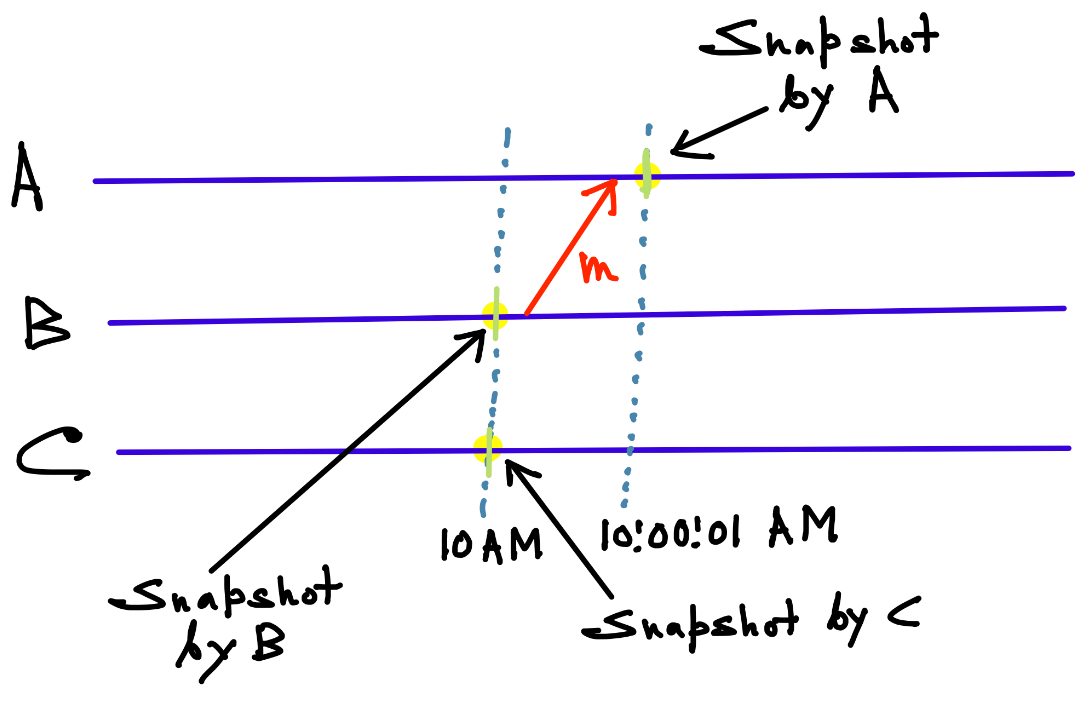
\includegraphics[width=0.5\textwidth]{IMG/Q2.jpeg}
    \caption{Timeline of Events}
    \label{fig:timeline}
\end{figure}

Let us analyze the snapshot operation at the reference time \(10{:}00{:}00\):  
\begin{itemize}
    \item At this time, the clock of node \(A\) displays \(09{:}59{:}59\).  
    \item The clocks of nodes \(B\) and \(C\) both display \(10{:}00{:}00\).  
\end{itemize}

Nodes \(B\) and \(C\) store their snapshots immediately at \(10{:}00{:}00\) (reference clock), whereas node \(A\) stores its snapshot when its clock reaches \(10{:}00{:}00\), which corresponds to the reference time \(10{:}00{:}01\).

Now, consider the following message-passing scenario:  
\begin{itemize}
    \item Node \(B\) sends a message \(m\) to node \(A\) just after the reference time \(10{:}00{:}00\).  
    \item Node \(A\) receives this message just before its clock reaches \(10{:}00{:}00\) (at reference time \(10{:}00{:}01\)).  
\end{itemize}

In this case:  
\begin{itemize}
    \item In the snapshot recorded by \(B\), the send event of message \(m\) will not be recorded. That is, \(\texttt{send}(m) \notin LS_B\).
    \item In the snapshot recorded by \(A\), the receive event of message \(m\) will be recorded. That is, \(\texttt{receive}(m) \in LS_A\).
\end{itemize}

Thus, the global snapshot will contain an inconsistency:  
\[
\texttt{inconsistent}(LS_B, LS_A) = \{m\}
\]
Since this set is not empty, the global snapshot is inconsistent.


% Include Problem 3
\section{Problem 3}\label{prob3}

Each node in the network stores the following information:
\begin{itemize}
    \item \textbf{Parent:} Initialized to \texttt{null}. (The parent node of the current node.)
    \item \textbf{Children:} Initialized to an empty list. (The list of child nodes of the current node.)
    \item \textbf{Forward Count:} Initialized to \texttt{0}. (The number of neighbors to whom the current node has forwarded a message asking to be its child.)
    \item \textbf{Reply Count:} Initialized to \texttt{0}. (The number of neighbors that have replied to the current node's request to be its child.)
    \item \textbf{ACK Count:} Initialized to \texttt{0}. (The number of children \(c\) of the current node that have informed that the spanning tree construction is complete for the subtree rooted at \(c\).)
\end{itemize}

Apart from the above information, each node also maintains a list of its neighbors. The neighbors are the nodes to which the current node is directly connected and can communicate with.

There are four types of messages in the protocol: \texttt{ASK}, \texttt{CHILD}, \texttt{REJ}, and \texttt{ACK}. Each node follows the rules below for handling each message type:

\subsection{Message Handling Rules}

\paragraph{On receiving an \texttt{ASK} message:}
\begin{enumerate}
    \item If the \texttt{Parent} is not \texttt{null}: 
    \begin{itemize}
        \item Send a \texttt{REJ} message to the sender. (The node is already connected to a parent. So, it rejects the request.)
    \end{itemize}
    \item Otherwise:
    \begin{itemize}
        \item Set the \texttt{Parent} to the sender. (The node accepts the sender as its parent.)
        \item Send a \texttt{CHILD} message to the sender. (The node informs the sender that it has accepted it as its child.)
        \item Send \texttt{ASK} messages to all other neighbors, excluding the sender. (The node asks all other neighbors to be its children.)
        \item Set \texttt{Forward Count} to the number of neighbors to whom the \texttt{ASK} message was sent. (The node sets the number of neighbors to which it has asked to be its children.)
    \end{itemize}
\end{enumerate}

\paragraph{On receiving a \texttt{REJ} message:}
\begin{enumerate}
    \item Increment the \texttt{Reply Count} by \texttt{1}. (The node received a rejection from a neighbor.)    
    \item If \(\texttt{Reply Count} = \texttt{Forward Count}\) and \(\texttt{ACK Count} = \texttt{Children.size()}\): (All neighbors have replied in response to the \texttt{ASK} message, and all children have informed that the spanning tree construction is complete for the subtree rooted at them.)
    \begin{itemize}
        \item Send an \texttt{ACK} message to the parent. (Send an acknowledgment to the parent indicating that the spanning tree construction is complete for the subtree rooted at the current node.)
    \end{itemize}
\end{enumerate}

\paragraph{On receiving a \texttt{CHILD} message:}
\begin{enumerate}
    \item Add the sender to the \texttt{Children} list. (The node accepted a child.)
    \item Increment the \texttt{Reply Count} by \texttt{1}.
    \item If \(\texttt{Reply Count} = \texttt{Forward Count}\) and \(\texttt{ACK Count} = \texttt{Children.size()}\): (All neighbors have replied in response to the \texttt{ASK} message, and all children have informed that the spanning tree construction is complete for the subtree rooted at them.)
    \begin{itemize}
        \item Send an \texttt{ACK} message to the parent. (Send an acknowledgment to the parent indicating that the spanning tree construction is complete for the subtree rooted at the current node.)
    \end{itemize}
\end{enumerate}

\paragraph{On receiving an \texttt{ACK} message:}
\begin{enumerate}
    \item Increment the \texttt{ACK Count} by \texttt{1}. (The node received an acknowledgment from a child indicating that the spanning tree construction is complete for the subtree rooted at the child.)
    \item If \(\texttt{Reply Count} = \texttt{Forward Count}\) and \(\texttt{ACK Count} = \texttt{Children.size()}\): (All neighbors have replied in response to the \texttt{ASK} message, and all children have informed that the spanning tree construction is complete for the subtree rooted at them.)
    \begin{itemize}
        \item Send an \texttt{ACK} message to the parent. (Send an acknowledgment to the parent indicating that the spanning tree construction is complete for the subtree rooted at the current node.)
    \end{itemize}
\end{enumerate}

\subsection{Initialization and Termination Conditions}

\paragraph{Initialization:}
The root node initializes the protocol by performing the following steps:
\begin{itemize}
    \item Send an \texttt{ASK} message to all its neighbors.
    \item Set its \texttt{Parent} to itself. (This ensures the root does not accept any other node as its parent.)
    \item Set \texttt{Forward Count} to the number of neighbors to whom the \texttt{ASK} message was sent.
\end{itemize}
Note: The root node does not add itself to its \texttt{Children} list, avoiding unnecessary self-messages.

\paragraph{Termination:}
The protocol terminates when the root node satisfies the following condition:
\[\texttt{Reply Count} = \texttt{Forward Count} \quad \text{and} \quad \texttt{ACK Count} = \texttt{Children.size()}.\]
This condition ensures that all neighbors have replied in response to the \texttt{ASK} message, and all children have informed that the spanning tree construction is complete for the subtree rooted at them.


% Include Problem 4
\section{Problem 4}\label{prob4}

The overall algorithm for the global snapshot consists of three main steps:
\begin{enumerate}
    \item \textbf{Spanning Tree Construction}
    \item \textbf{Recording Snapshots at Each Node}
    \item \textbf{Propagating Snapshots to the Root Node through the Spanning Tree}
\end{enumerate}

\subsection{Spanning Tree Construction}
For constructing the spanning tree, we use the algorithm discussed in question \ref{prob3}, with slight modifications to leverage the synchronous nature of the links and reduce the number of messages. Specifically:
\begin{itemize}
    \item The \texttt{REJ} message is eliminated, and instead, a timeout mechanism is employed to detect cases where a node has already been connected to a parent.
    \item Further optimization, such as eliminating the \texttt{ACK} message, could be achieved if the network's diameter were known. While a bound on the diameter can be indirectly derived as \(n-1\) (given a bound on the number of nodes \(n\)), we skip this optimization as it is not explicitly stated in the problem.
\end{itemize}

\noindent The modified algorithm for constructing the spanning tree is as follows:

Each node in the network stores the following information:
\begin{itemize}
    \item \textbf{Parent:} Initialized to \texttt{null}. (The parent node in the spanning tree.)
    \item \textbf{Children:} Initialized to an empty list. (The list of children in the spanning tree.)
    \item \textbf{ACK Count:} Initialized to \texttt{0}. (The number of acknowledgments received from children \(c\) indicating that the spanning tree construction is complete for the subtree rooted at \(c\).)
\end{itemize}

There are three types of messages in the protocol: \texttt{ASK}, \texttt{CHILD}, and \texttt{ACK}. Each node follows the rules below for handling each message type:

\subsubsection{Message Handling Rules}

\paragraph{On receiving an \texttt{ASK} message:}
\begin{enumerate}
    \item If the \texttt{Parent} is not \texttt{null}: (The node is already connected to a parent.)
    \begin{itemize}
        \item Ignore the message. (No action is taken. The rejection is implicit because of timeout.)
    \end{itemize}
    \item Otherwise:
    \begin{itemize}
        \item Set the \texttt{Parent} to the sender. (The node accepts the sender as its parent.)
        \item Send a \texttt{CHILD} message to the sender. (The sender is accepted as a child.)
        \item Send a \texttt{ASK} message to all other neighbors, excluding the sender. Start a timer for the \texttt{ASK} message with duration \(2\times T\). (The node ask its neighbors to become its children. It also sets a timer with maximum round-trip time. Any node not responding within this time to the \texttt{ASK} message does not become a child.)
    \end{itemize}
\end{enumerate}

\paragraph{On receiving a \texttt{CHILD} message:}
\begin{enumerate}
    \item Add the sender to the \texttt{Children} list. (The node accepted a child.)
    \item If \(\texttt{ACK Count} = \texttt{Children.size()}\) and the timer has expired: (All children have informed the node that the spanning tree construction is complete for their subtrees and the timer has expired)
    \begin{itemize}
        \item Send an \texttt{ACK} message to the parent. (All children have acknowledged.)
    \end{itemize}
\end{enumerate}

\paragraph{On receiving an \texttt{ACK} message:}
\begin{enumerate}
    \item Increment the \texttt{ACK Count} by \texttt{1}. (The node received an acknowledgment from a child indicating that the spanning tree construction is complete for the subtree rooted at the child.)
    \item If \(\texttt{ACK Count} = \texttt{Children.size()}\) and the timer has expired: (All children have acknowledged and the timer has expired)
    \begin{itemize}
        \item Send an \texttt{ACK} message to the parent. (Send an acknowledgment to the parent indicating that the spanning tree construction is complete for the subtree rooted at the node.)
    \end{itemize}
\end{enumerate}

\subsubsection{Timeout Handling}
If the timer for the \texttt{ASK} message expires, the node proceeds as follows: (Within, this time, the node expects a \texttt{CHILD} message from the neighbor which has accepted the node as a parent.)
\begin{enumerate}
    \item If \(\texttt{ACK Count} = \texttt{Children.size()}\): (All children have acknowledged that the spanning tree construction is complete for their subtrees.)
    \begin{itemize}
        \item Send an \texttt{ACK} message to the parent. (Send an acknowledgment to the parent indicating that the spanning tree construction is complete for the subtree rooted at the node.)
    \end{itemize}
\end{enumerate}

\subsubsection{Initialization and Termination Conditions}
A node \(i\) begins the spanning tree construction by:
\begin{itemize}
    \item Sending an \texttt{ASK} message to all its neighbors. (The node asks its neighbors to become its children.)   
    \item Setting itself as the root node for its local state. (The node is the root of the spanning tree.)
    \item Starting a timer for the \texttt{ASK} message with a duration of \(2 \times T\). (The node sets a timer with maximum round-trip time. Any node not responding within this time to the \texttt{ASK} message does not become a child.)
\end{itemize}

The spanning tree construction is considered complete at node \(i\) when the following conditions are met:
\begin{itemize}
    \item The \texttt{ACK Count} equals the size of its \texttt{Children} list. (All children have acknowledged that the spanning tree construction is complete for their subtrees.)
    \item The timer has expired. (The timer for the \texttt{ASK} message has expired.)
\end{itemize}

\subsection{Recording Snapshots at Each Node}

To record snapshots at each node, we modify the Chandy-Lamport algorithm to handle non-FIFO channels. To do this, we introduce a delay after sending the marker message to ensure that all messages sent before the marker message are received.

Each node in the network maintains the following information:

\begin{itemize}
    \item \textbf{Local State:} Stores the state of the node, initially set to \texttt{null}.
    \item \textbf{Channel States:} For each neighbor, stores the state of the channel directed to the node. Specifically, for each neighbor \(j\), the node maintains the state of the channel from \(j\) to itself. All channel states are initialized to \texttt{null}.
\end{itemize}

When node \(x\) receives a marker message from a neighbor \(y\) along the channel \(y \rightarrow x\), the following steps are executed:

\begin{enumerate}
    \item \textbf{If the node has not recorded its local state:}
    \begin{itemize}
        \item Upon receiving the marker message, wait for \(T\) time units to detect any pending messages. If any pending messages are detected, process them and accordingly update the local state. (This step ensures that all messages sent before the marker message are received and processed.)
        \item Record the local state of the node as the state at the end of the waiting period. Record the state of the channel \(y \rightarrow x\) as empty. (The channel state is recorded as empty since the marker message is the last message sent along the channel.)
        \item Send marker messages to all neighbors. (The node sends marker messages to all neighbors asking them to record their local states.)
        \item After sending the marker messages, delay sending any further messages for \(2 \times T\) time units, i.e., wait for \(2 \times T\) time units before placing any new messages in the channels. (This delay ensures that the receiving node can differentiate between messages sent before and after the marker message.)
    \end{itemize}
    
    \item \textbf{If the node has already recorded its local state:}
    \begin{itemize}
        \item Let \(M_1\) denote the set of messages received before the marker message from \(y\) and after the local state was recorded by \(x\). (These messages are received after the local state was recorded but before the marker message was received.)
        \item Upon receiving the marker message, the node waits for \(T\) time units to detect any pending messages. Let \(M_2\) represent the set of messages received during this waiting period from \(y\). (These messages are received after the marker message was received and during the waiting period.)
        \item Record the state of the channel \(y \rightarrow x\) as \(M_1 \cup M_2\), the union of the two sets of messages. 
    \end{itemize}
\end{enumerate}

In order to see how we use the timeouts value to differentiate between messages sent before and after the marker message, consider the following scenario:(All the time values are with respect to a global reference clock.)

A node $x$ sends a marker message $M$ to a neighbor $y$ at time $t_M = t_1$. The message is received by $y$ at time $t_{rec}^{(M)} \in [t_1, t_1+T]$. Since our algorithm does not restrict sending messages before the marker, assume that $x$ sent another message $msg$ to $y$ at time $t_{msg} = t_1 - \epsilon$, where $\epsilon$ is a small positive value. This message is received by $y$ at time $t_{rec}^{(msg)} \in [t_1 - \epsilon, t_1 + T - \epsilon]$. In the worst case, it is possible that $t_{rec}^{(M)} = t_1$ while $t_{rec}^{(msg)} = t_1 + T - \epsilon$. As a result, after receiving the marker message, $y$ must wait for $T$ time units to detect any pending messages.

% Inserting the figure
\begin{figure}[h]
    \centering
    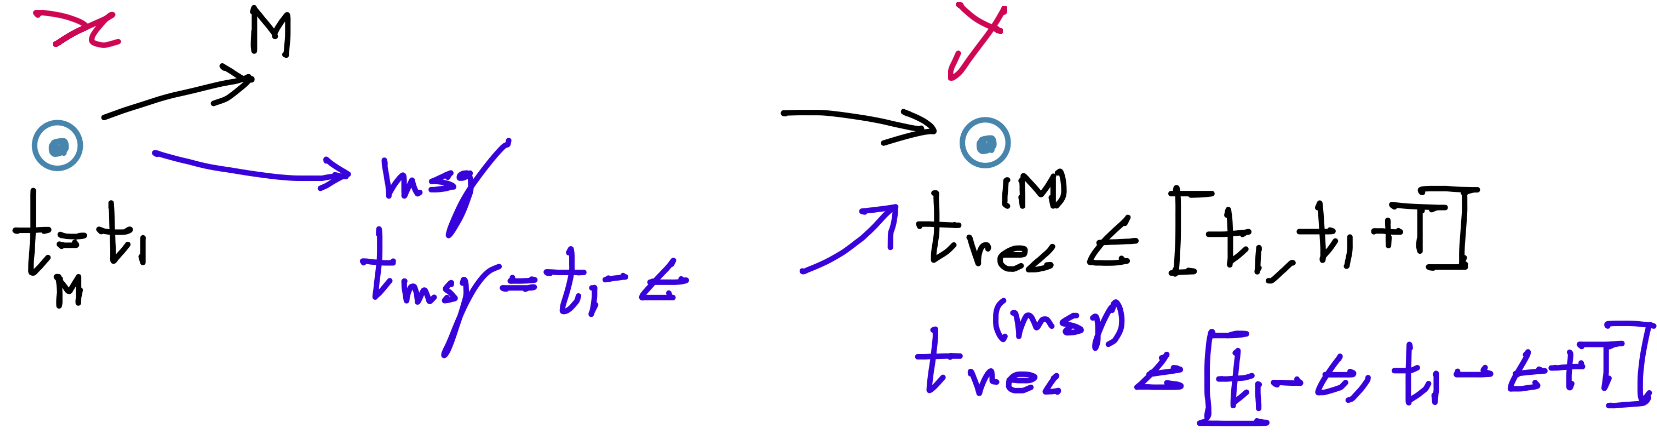
\includegraphics[width=0.8\textwidth]{IMG/Q4.jpeg}
    \caption{Illustration of the timeout mechanism for recording snapshots}
    \label{fig:fig1}
\end{figure}

Since $y$ is unaware of the delay for the marker message, it must wait $T$ time units irrespective of the marker's delay to detect any pending messages. If the marker message is delayed by $T$ time units, $y$ will still have to wait for $T$ time units to detect any pending messages after the marker's receive. In the worst case, $y$ may have to wait until $t_1 + 2T$ to identify any pending messages. After this period, any message received by $y$ is considered to have been sent after the marker message. This justifies our algorithm's requirement that $x$ must wait for $2 \times T$ time units before placing any new messages in the channel.


\subsubsection{Initialization and Termination Conditions}

The global snapshot algorithm is initiated by a node \(i\) through the following steps:
\begin{itemize}
    \item The node first records its local state.
    \item It then sends marker messages to all its neighbors.
    \item After sending the marker messages, the node waits for \(2 \times T\) time units before placing any new messages in the channel.
\end{itemize}


A local state recording of a node is deemed complete when both the node's state and all its incoming channel states have been recorded. This condition will eventually be satisfied for all nodes in the network, as the graph is connected. 

At this stage, we will not detect the completion of the global snapshot but we note here that each node can independently detect the completion of its local snapshot recording. We will now use the spanning tree constructed in the previous step to propagate the snapshots to the root node.

\subsection{Propagating Snapshots to the Root Node through the Spanning Tree}
As we noted, every node can independently detect the completion of its local snapshot recording. The next step is to propagate the snapshots to the root node through the spanning tree. The idea is to send the snapshots from the leaf nodes to the root node, merging the snapshots as they propagate upwards. A node can send the snapshot to its parent only when it has received snapshots from all its children and has recorded its local state. The message format can be defined as follows where we assume that the snapshot is a JSON object: (The format of the snapshot can be modified based on the requirements of the application. The only requirement is that the receiver and sender agree on the format.)

\begin{verbatim}
{
    "node_id": <node_id>,
    "local_state": <local_state>,
    "channel_states": {
        "link_1": <state>,
        "link_2": <state>,
        ...
    }
}
\end{verbatim}

Each node \(j\) in the network maintains the following information:
\begin{itemize}
    \item \textbf{Snapshot State:} Initially set to \texttt{null}.
    \item \textbf{Received Snapshots:} A list of snapshots received from all children, initially set to an empty list.
\end{itemize}

When node \(j\) receives a snapshot from a child \(i\) or detects that its local state and channel states have been recorded, it follows the steps below:

\begin{enumerate}
    \item If the snapshot is received from a child \(i\), add it to the \texttt{Received Snapshots} list. (The snapshot received from child \(i\) is added to the list of received snapshots.)
    \item If the size of the \texttt{Received Snapshots} list equals the number of children of node \(j\), and the local state and channel states of node \(j\) have been recorded: (All children have sent snapshots from their subtrees, and the local state and channel states of node \(j\) have been recorded.)
    \begin{itemize}
        \item Merge the local state of node \(j\) with the channel states of node \(j\), along with the snapshots received from all children. (The local state and channel states of node \(j\) are merged with the snapshots received from all children.)
        \item Send the merged snapshot to the parent of node \(j\). (The merged snapshot is sent to the parent of node \(j\).)
    \end{itemize}
\end{enumerate}

The node \(i\) that initiated the global snapshot can detect its completion once it receives a snapshot from all its children in the spanning tree. The snapshot received by the root node is the global snapshot of the network.

\subsection{Message Complexity}

Let \(n\) be the number of nodes in the network and \(m\) be the number of channels. The message complexity of the global snapshot algorithm can be analyzed as follows:

\begin{enumerate}
    \item \textbf{Spanning Tree Construction:} During the spanning tree construction, each node sends at most one \texttt{ASK} message to each of its neighbors. This results in atmost \(2 \times m\) messages. Additionally, the \texttt{CHILD} and \texttt{ACK} messages are sent in response from child to parent, each being sent \(n-1\) times. Therefore, the total number of messages sent during spanning tree construction is:
    \[
    2 \times (m + n - 1)
    \]
    
    \item \textbf{Recording Snapshots at Each Node:} The marker message is sent along each channel at most twice, so the number of messages sent during snapshot recording is at most:
    \[
    2 \times m
    \]
    
    \item \textbf{Propagating Snapshots to the Root Node:} The number of messages sent during the propagation of snapshots to the root node is \(n-1\).
\end{enumerate}

Summing the message complexities of these three steps, the total message complexity of the global snapshot algorithm is:
\[
2 \times (m + n - 1) + 2 \times m + (n - 1) = 4 \times m + 3 \times n - 3 = O(m + n)
\]



% Include Problem 5
\section{Problem 5}\label{prob5}

In this problem, we modify the Ricart-Agrawala algorithm to design a permission-based distributed mutual exclusion algorithm that requires zero messages in the best case.

\subsection{Best-Case Scenario}
The best case occurs when a single process repeatedly requests access to the critical section while no other process makes a request. The key idea is that once a process \( p_i \) has received a \texttt{REPLY} message from another process \( p_j \), it does not need to send a \texttt{REQUEST} message to \( p_j \) again unless \( p_i \) has sent a \texttt{REPLY} message to \( p_j \) in response to a \texttt{REQUEST}. Consequently, if only one process requests the critical section, it initially needs to obtain permission from all other processes. However, subsequent requests will not require any additional messages since permission has already been acquired.

Additionally, if a subset of processes requests the critical section, only the processes within the subset need to communicate with each other once all other processes have granted permission at least once to each process in the subset.

\subsection{Worst-Case Scenario}
The worst case arises when all processes frequently request access to the critical section. In this scenario, any process \( p_i \) cannot hold permission indefinitely, as it must send \texttt{REPLY} messages to other processes upon receiving their \texttt{REQUEST} messages. As a result, each new request necessitates sending a \texttt{REQUEST} message to all other processes and waiting for their \texttt{REPLY} messages. This scenario requires \( 2(N-1) \) messages per request in the worst case.

\subsection{Process State Management}
Each node maintains a logical clock updated following the Lamport clock rules, along with the following data structures:

\begin{itemize}
    \item \textbf{Request Queue:} A queue of requests for the critical section, ordered by logical timestamps.
    \item \textbf{Permission Array:} A boolean array of size \( N \), where the \( i \)-th element is \texttt{true} if process \( p_i \) has granted permission to the current process and \texttt{false} otherwise. Initially, all elements are set to \texttt{false} except for the current process's index, which is \texttt{true}.
    \item \textbf{My Requests Queue:} A list of requests sent by the current process, ordered by logical timestamps.
\end{itemize}

\subsection{Message Types}
The system uses two types of messages:
\begin{itemize}
    \item \texttt{REQUEST(i, ts)}: Sent by process \( p_i \) to request access to the critical section, where \( ts \) is the logical timestamp.
    \item \texttt{REPLY(i)}: Sent by process \( p_i \) to grant permission to another process.
\end{itemize}

\subsection{Requesting the Critical Section}
To request critical section access, process \( p_i \) follows these steps:

\begin{enumerate}
    \item If the request queue is empty and all elements of the permission array are \texttt{true}, enter the critical section (no communication needed).
    \item Otherwise, send a \texttt{REQUEST(i, ts)} message to all processes for which the corresponding element of the permission array is \texttt{false}. Add the request to both the \texttt{Request Queue} and \texttt{My Requests Queue}. It will eventually enter the critical section when all elements of the permission array are \texttt{true}.
\end{enumerate}

\subsection{Handling a \texttt{REQUEST} Message}
Upon receiving a \texttt{REQUEST(i, ts)} message from process \( p_i \), process \( p_j \) executes the following steps:

\begin{enumerate}
    \item If \( p_j \) is not interested in the critical section (i.e., \texttt{My Requests Queue} is empty and it is not currently in the critical section), it:
    \begin{itemize}
        \item Sends a \texttt{REPLY(j)} message to \( p_i \).
        \item Sets the \( i \)-th element of the permission array to \texttt{false}.
    \end{itemize}
    
    \item If \( p_j \) is currently in the critical section, it adds the request to the \texttt{Request Queue} for later processing.
    
    \item If \( p_j \) is interested in the critical section (but not currently executing), it compares the timestamp of the received request with the request at the front of \texttt{My Requests Queue}:
    \begin{itemize}
        \item If the received request has a smaller timestamp, \( p_j \) does the following:
        \begin{itemize}
            \item Sends a \texttt{REPLY(j)} message to \( p_i \).
            \item Sets the \( i \)-th element of the permission array to \texttt{false}.
            \item If the \( i \)-th element of the permission array was previously \texttt{true}, it also sends a \texttt{REQUEST(j, ts\_{\text{front}})} message to \( p_i \) to inform \( p_i \) of its own request, where \texttt{ts\_{\text{front}}} is the timestamp of the request at the front of \texttt{My Requests Queue}.
        \end{itemize}
    \end{itemize}
\end{enumerate}


\subsection{Handling a \texttt{REPLY} Message} \label{prob5:reply}
Upon receiving a \texttt{REPLY(j)} message from process \( p_j \), process \( p_i \):
\begin{enumerate}
    \item Sets the \( j \)-th element of the permission array to \texttt{true}.
    \item If a request from \(p_i\) is present in the \texttt{My Requests Queue}, it checks if all elements of the permission array are \texttt{true}. If so, it enters the critical section and removes its request from both the \texttt{Request Queue} and \texttt{My Requests Queue}.
    \item Otherwise, it waits for more \texttt{REPLY} messages.
\end{enumerate}

\subsection{Releasing the Critical Section}
To release the critical section, process \( p_i \):
\begin{enumerate}
    \item Sends a \texttt{REPLY(i)} message to all processes in the \texttt{Request Queue}.
    \item Sets the corresponding elements of the permission array to \texttt{false}.
    \item Removes the requests from the \texttt{Request Queue}.
\end{enumerate}


% Include Problem 6
\section{Problem 6}\label{prob6}

To construct a BFS spanning tree, we use an algorithm similar to the one described in Problem \ref{prob3}, but with modified message types and handling rules to ensure the BFS property rather than an arbitrary spanning tree.

\subsection{Node Data Structure}
Each node in the network maintains the following information:
\begin{itemize}
    \item \textbf{Parent:} Initially set to \texttt{null}. (The node's parent in the BFS spanning tree.)
    \item \textbf{Children:} Initially an empty list. (The node's children in the BFS spanning tree.)
    \item \textbf{Forward Count:} Initially \texttt{0}. (Number of neighbors to which the node sent an \texttt{ASK}/\texttt{JOIN} message.)
    \item \textbf{Reply Count:} Initially \texttt{0}. (Number of replies received by the node.)
    \item \textbf{Level:} Initially \texttt{0}. (The node's level in the BFS spanning tree.)
    \item \textbf{New Node Found:} Initially \texttt{false}. (Flag indicating if a new node was added to the subtree rooted at the node during a phase.)
\end{itemize}

\subsection{Message Types}
The protocol utilizes the following message types:
\begin{itemize}
    \item \texttt{JOIN(LEVEL)}: Sent by the root to initiate the expansion to level \texttt{LEVEL}.
    \item \texttt{ASK(LEVEL)}: Sent by a node at level \texttt{LEVEL-1} to its neighbors asking them to join level \texttt{LEVEL}.
    \item \texttt{ACK}: Acknowledgment message sent by a node to its parent when it agrees to join the tree.
    \item \texttt{NACK}: Negative acknowledgment message sent by a node when it is already part of the tree.
    \item \texttt{DONE(LEVEL,NEW\_NODE\_FOUND)}: Sent by a node to its parent to indicate completion of level \texttt{LEVEL} in its subtree. The \texttt{NEW\_NODE\_FOUND} field is set to \texttt{true} if at least one new node was added to the tree.
\end{itemize}

\subsection{Algorithm Description}
Let's say at any phase \( i \), the BFS spanning tree has been constructed up to level \( i \), and termination has been detected by the root for this level. We now describe the process of expanding the tree to level \( i+1 \).

\begin{figure}[h]
    \centering
    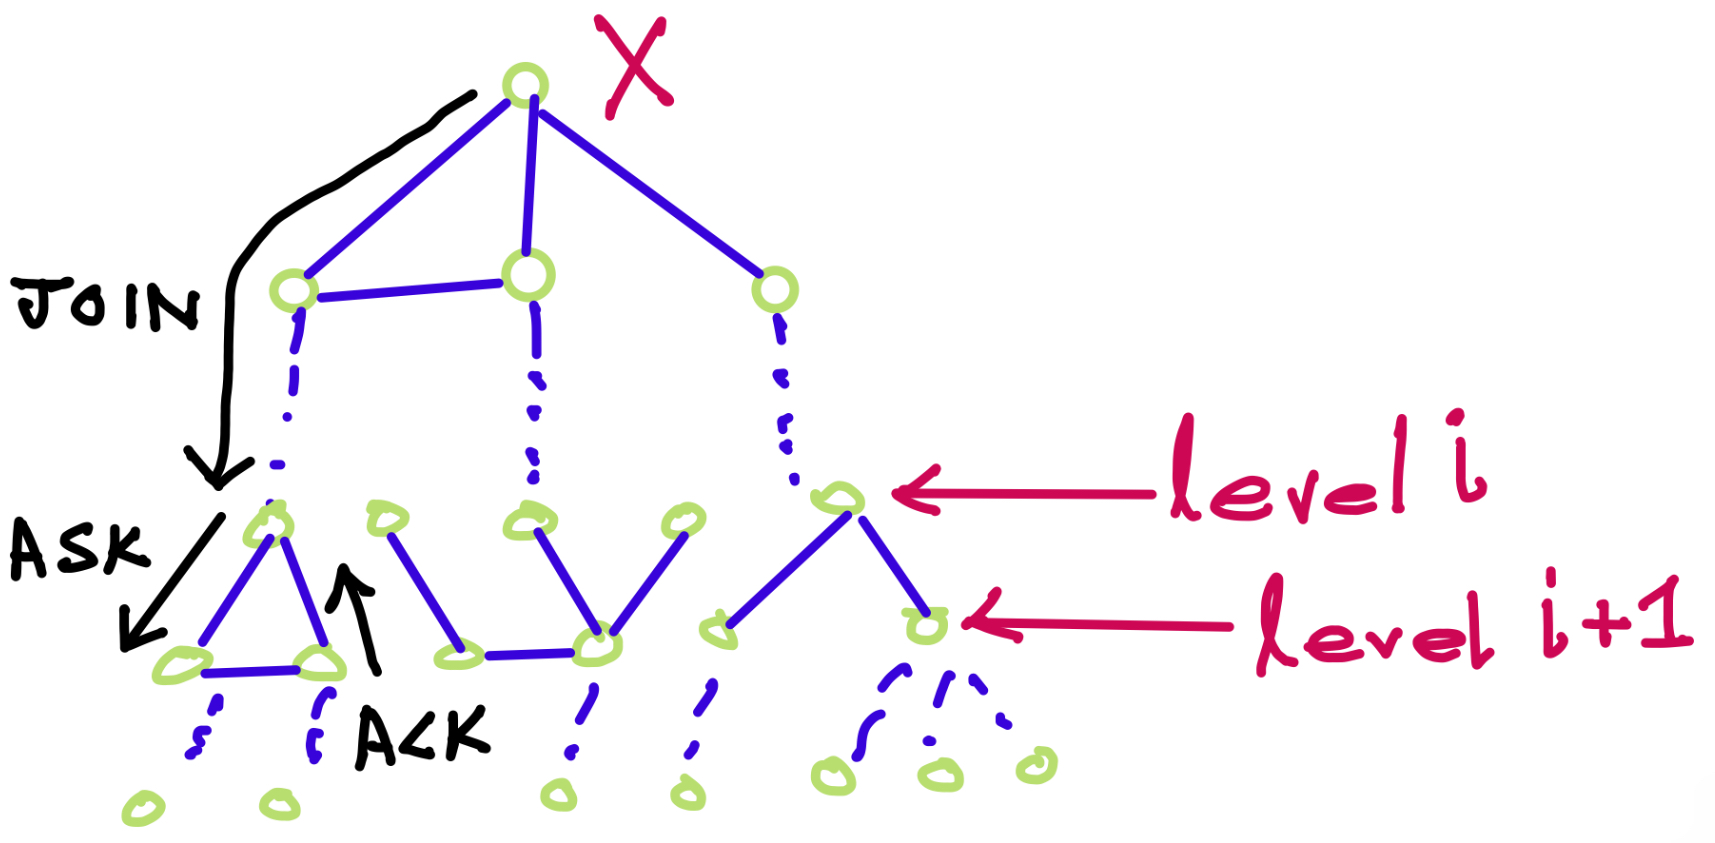
\includegraphics[width=0.5\textwidth]{IMG/Q6.jpeg}
    \caption{Expansion of the BFS Spanning Tree to Level \( i+1 \).}
    \label{fig:BFS}
\end{figure}

\subsubsection{Step 1: Sending JOIN Messages}
The root node initiates the process by sending a \texttt{JOIN(i+1)} message to all its \texttt{Children}. Any node \( u \) at level \( j \) (\( j < i \)) forwards this message to all its \texttt{Children}.

\subsubsection{Step 2: ASK and ACK/NACK Exchange}
When a node at level \( i \) receives \texttt{JOIN(i+1)}, it sends an \texttt{ASK(i+1)} message to all directly connected nodes except its \texttt{Parent}. It also sets:
\begin{itemize}
    \item \texttt{Forward Count} to the number of nodes to which it sent \texttt{ASK}.
    \item \texttt{Reply Count} to \texttt{0}.
\end{itemize}

Nodes that receive \texttt{ASK(i+1)} respond as follows:
\begin{itemize}
    \item If already part of the spanning tree, they send a \texttt{NACK}.
    \item If not part of the tree and receiving \texttt{ASK} for the first time:
    \begin{itemize}
        \item They send an \texttt{ACK}.
        \item They mark the sender as their \texttt{Parent} and set their \texttt{Level} to \( i+1 \).
    \end{itemize}
\end{itemize}

Nodes at level \( i \) collect \texttt{ACK} and \texttt{NACK} responses, updating:
\begin{itemize}
    \item \textbf{Children:} Nodes from which they receive \texttt{ACK}.
    \item \textbf{Reply Count:} Increments for every received \texttt{ACK} or \texttt{NACK}.
\end{itemize}

\subsubsection{Step 3: Propagating DONE Messages}
Once a node at level \( i \) has received replies from all nodes it sent \texttt{ASK} to (\texttt{Forward Count} = \texttt{Reply Count}), it sends a \texttt{DONE(LEVEL,NEW\_NODE\_FOUND)} message to its \texttt{Parent}. Here, \texttt{NEW\_NODE\_FOUND} is:
\begin{itemize}
    \item \texttt{true} if at least one \texttt{ACK} was received.
    \item \texttt{false} otherwise.
\end{itemize}

Nodes at top levels \( j\) \((j < i \)) wait for \texttt{DONE} messages from all their \texttt{Children} before forwarding the \texttt{DONE} message to their own \texttt{Parent}. The \texttt{NEW\_NODE\_FOUND} field is set to \texttt{true} if at least one child reported \texttt{NEW\_NODE\_FOUND = true}.

\subsubsection{Step 4: Root Detection of Termination}
The root node \(X\) receives \texttt{DONE} messages from all its \texttt{Children}. If any contain \texttt{NEW\_NODE\_FOUND = true}, it proceeds to phase \( i+2 \). Otherwise, the algorithm terminates, completing the BFS spanning tree construction.

This process can be repeated until the root detects that no new nodes were added to the tree in the last phase, signaling the completion of the BFS spanning tree.

\subsection{Message Handling Rules}

\subsubsection{Handling a \texttt{JOIN} Message}
When a node receives a \texttt{JOIN(i)} message:
\begin{itemize}
    \item If the node is at level \( i - 1 \), it sends an \texttt{ASK(i)} message to all its neighbors except the \texttt{Parent} and sets \texttt{New Node Found} to \texttt{false}. It also set the \texttt{Forward Count} to the number of neighbors to which it sent the message and \texttt{Reply Count} to \texttt{0}. (Nodes that are leaves in the current treen send \texttt{ASK} messages to all their neighbors asking them to join level \( i \).)
    \item If the node is at level \( j < i - 1 \), it forwards the message to all its \texttt{Children} and sets \texttt{Reply Count} to \texttt{0}. (Nodes that are not leaves in the current tree forward the \texttt{JOIN} message to their children.)
\end{itemize}

\subsubsection{Handling an \texttt{ASK} Message}
Upon receiving an \texttt{ASK(i)} message:
\begin{itemize}
    \item If the \texttt{Parent} field is not \texttt{null}, reply with a \texttt{NACK} message. (The node is already part of the BFS spanning tree.)
    \item Otherwise, reply with an \texttt{ACK} message, set the \texttt{Parent} field to the sender, and \texttt{Level} to \( i \). (The node joins the BFS spanning tree at level \( i \).)
\end{itemize}

\subsubsection{Handling an \texttt{ACK} Message}
Upon receiving an \texttt{ACK} message:
\begin{itemize}
    \item Add the sender to the \texttt{Children} list. (The sender is now a child of the node.)
    \item Increment the \texttt{Reply Count}. (The node has received a reply.)
    \item If \texttt{Reply Count} = \texttt{Forward Count}, send a \texttt{DONE(Level,true)} message to the \texttt{Parent}. (All replies have been received from the neighbors.)
\end{itemize}

\subsubsection{Handling a \texttt{NACK} Message}
Upon receiving a \texttt{NACK} message:
\begin{itemize}
    \item Increment the \texttt{Reply Count}. (The node has received a reply.)
    \item If \texttt{Reply Count} = \texttt{Forward Count}, check if the \texttt{Children} list is empty. If so, send a \texttt{DONE(level,false)} message to the \texttt{Parent}. Otherwise, send a \texttt{DONE(level,true)} message to the \texttt{Parent}. (All replies have been received from the neighbors. If no new nodes were explored, the \texttt{NEW\_NODE\_FOUND} field is set to \texttt{false}.)
\end{itemize}

\subsubsection{Handling a \texttt{DONE} Message}
Upon receiving a \texttt{DONE(i,NEW\_NODE\_FOUND)} message:
\begin{itemize}
    \item Increment the \texttt{Reply Count}. (The node has received a \texttt{DONE} message from a child indicating BFS tree construction up to level \( i \) in the child's subtree.)
    \item Set \texttt{New Node Found} to \( \texttt{New Node Found} \vee \texttt{NEW\_NODE\_FOUND} \). (Update the \texttt{New Node Found} flag based on the child's message.)
    \item If \texttt{Reply Count} = \texttt{Forward Count}, send a \texttt{DONE(i,New Node Found)} message to the \texttt{Parent}. (All replies have been received from the children. Send a message to the parent indicating completion of level \( i \) in the subtree.)
\end{itemize}


\subsection{Initialization and Termination}
The root node \( X \) initiates the BFS spanning tree construction by sending a \texttt{JOIN(1)} message to all its \texttt{Children}. It also sets itself as the root of the tree by setting its \texttt{Parent} field to \(X\) and \texttt{Level} to \(0\).

For each phase \( i \), the root sends a \texttt{JOIN(i)} message to all its \texttt{Children} and waits for \texttt{DONE(i, NEW\_NODE\_FOUND)} messages from all of them. If at least one \texttt{DONE} message contains \texttt{NEW\_NODE\_FOUND = true}, the process continues to phase \( i+1 \). Otherwise, the algorithm terminates, signaling the completion of the BFS spanning tree.

\subsection{Message Complexity}
Let \( N \) represent the number of nodes in the network, \( M \) the number of edges, and \( D \) the diameter.

The number of rounds is bounded by the network's diameter. For each edge \( (u, v) \), the \texttt{ASK} and \texttt{ACK}/\texttt{NACK} messages are exchanged at most twice, resulting in a maximum of 4 messages per edge, leading to \( 4 \times M \) messages in total.

In each round, \texttt{JOIN} and \texttt{DONE} messages are exchanged across the tree edges, with a total of at most \( 2 \times (N-1) \) messages per round. Hence, the overall message complexity is:
\[
O(N \times D + M).
\]



% Include Problem 7
\section{Problem 7}\label{prob7}

This section describes the protocol for constructing a Depth-First Search (DFS) spanning tree in a network. The protocol uses a DFS traversal approach, with tie-breaking based on root node IDs in cases of concurrent initiation. Specifically, if multiple nodes initiate the process simultaneously, a node joins the tree rooted at the highest ID node in case of a conflict. The protocol employs the following message types and rules.

\subsection{Node Data Structure}
Each node in the network maintains the following data:
\begin{itemize}
    \item \textbf{Parent}: Initially set to \texttt{null}. (Represents the parent node in the DFS tree.)
    \item \textbf{MyRoot}: Initially set to \texttt{null}. (Represents the root node of the DFS tree.)
    \item \textbf{Children}: An initially empty list to store child nodes. (These are nodes that have accepted the tree edge from the current node.)
    \item \textbf{Neighbors}: A list of adjacent nodes. (Represents the set of nodes directly connected to the current node.)
    \item \textbf{Unknown}: Initially set to the list of neighbors. (Represents nodes whose status is unknown i.e not yet visited in the DFS traversal.)
\end{itemize}

\subsection{Message Types}
The protocol uses the following message types:
\begin{itemize}
    \item \texttt{QUERY(id)}: Sent by a node to its neighbors to invite them to join the DFS tree rooted at the node with ID \texttt{id}.
    \item \texttt{ACCEPT(id)}: Sent by a node to its parent to confirm the acceptance of the tree edge. The \texttt{id} field contains the root node's ID.
    \item \texttt{REJECT(id)}: Sent by a node to its parent to decline the tree edge. The \texttt{id} field contains the root node's ID.
\end{itemize}

The \texttt{QUERY} messages facilitate the continuation of the DFS traversal from the current node. The \texttt{REJECT} message serves to detect cycles during the tree construction process. The \texttt{ACCEPT} message confirms the acceptance of a tree edge and notifies the parent node that all its neighbors have been visited. 

Additionally, if a node receives a \texttt{QUERY} message from a node with a higher root ID, it updates its tree membership to join the tree rooted at the higher ID node.

\subsection{Message Handling Rules}

\subsubsection{Handling a \texttt{QUERY} Message}
When a node \(i\) receives a \texttt{QUERY(id)} message from a neighbor \(j\), it performs the following steps:
\begin{enumerate}
    \item If \texttt{MyRoot} is \texttt{null} or \texttt{id} is greater than \texttt{MyRoot}: (The current node should join the tree rooted at \texttt{id}.)
    \begin{itemize}
        \item Set \texttt{MyRoot} to \texttt{id}. (Update the root node.)
        \item Set \texttt{Parent} to \(j\). (Set the parent node.)
        \item Set \texttt{Unknown} to the list of neighbors excluding \(j\). (Initialize the unknown list.)
        \item If \texttt{Unknown} is empty, send an \texttt{ACCEPT(id)} message to \(j\). (No unknown neighbors remain. So, accept the tree edge and notify the parent that DFS in the subtree is complete.)
        \item Otherwise, send a \texttt{QUERY(id)} message to the first node in \texttt{Unknown} and remove it from \texttt{Unknown}. (Continue DFS traversal by querying the next unknown neighbor.)
    \end{itemize}
    \item If \texttt{id} equals \texttt{MyRoot}, send a \texttt{REJECT(id)} message to \(j\). (Reject the tree edge if the root ID matches the current root. The node is already part of the same tree.)
    \item If \texttt{id} is less than \texttt{MyRoot}, ignore the message. (Reject the tree edge if the root ID is lower than the current root; the node is already part of a tree rooted at a higher ID.)
\end{enumerate}

\subsubsection{Handling an \texttt{ACCEPT} Message}
When a node \(i\) receives an \texttt{ACCEPT(id)} message from a neighbor \(j\), it performs the following steps:
\begin{enumerate}
    \item If \texttt{MyRoot} is \texttt{id}:
    \begin{itemize}
        \item Add \(j\) to the \texttt{Children} list. (Update the list of children.)
        \item If \texttt{Unknown} is empty:
        \begin{itemize}
            \item If \texttt{Parent} is \(i\), designate \(i\) as the root and terminate. (The current node is the root of the tree and all neighbors have been visited.)
            \item Otherwise, send an \texttt{ACCEPT(id)} message to \texttt{Parent}. (Notify the parent that all neighbors have been visited in the subtree.)
        \end{itemize}
        \item Otherwise, send a \texttt{QUERY(id)} message to the first node in \texttt{Unknown} and remove it from \texttt{Unknown}. (Continue DFS traversal by querying the next unknown neighbor.)
    \end{itemize}
    \item If \texttt{MyRoot} is not \texttt{id}, ignore the message. (This node has changed tree membership after sending the \texttt{QUERY} message.)
\end{enumerate}

\subsubsection{Handling a \texttt{REJECT} Message}
When a node \(i\) receives a \texttt{REJECT(id)} message from a child \(j\), it performs the following steps:
\begin{enumerate}
    \item If \texttt{MyRoot} is \texttt{id}:
    \begin{itemize}
        \item If \texttt{Unknown} is empty:
        \begin{itemize}
            \item If \texttt{Parent} is \(i\), designate \(i\) as the root and terminate. (The current node is the root of the tree and all neighbors have been visited.)
            \item Otherwise, send an \texttt{ACCEPT(id)} message to \texttt{Parent}. (Notify the parent that all neighbors have been visited in the subtree.)
        \end{itemize}
        \item Otherwise, send a \texttt{QUERY(id)} message to the first node in \texttt{Unknown} and remove it from \texttt{Unknown}. (Continue DFS traversal by querying the next unknown neighbor.)
    \end{itemize}
    \item If \texttt{MyRoot} is not \texttt{id}, ignore the message. (The node has changed tree membership after sending the \texttt{QUERY} message.)
\end{enumerate}

\subsection{Initialization and Termination}
To initiate the tree construction, a node \(i\) first checks if \texttt{Parent} is \texttt{null}. If so, it sends a \texttt{QUERY(i)} message to itself. (This is an internal action and does not involve actual communication.)

The tree construction terminates when the root node confirms that all its neighbors have been visited. This occurs when the \texttt{Unknown} list becomes empty. At this point, the root node designates itself as the root of the tree and finalizes the tree construction. To disseminate this information, the root node can propagate a completion signal throughout the spanning tree.

% Include Problem 8
\section{Problem 8}\label{prob8}

For this problem, we will utilize the concept that a request made by a node will be forwarded along the path directed by the \texttt{to\_token} value. Each node will make requests to the its parent, either for itself or on behalf of its subtree. The root is the node that holds the token. To allow access to the critical section, the token will be forwarded to the node with the earliest request in the queue. 

Additionally, depending on the forwarding of the token, the edges of the spanning tree will be reversed to point to the token holder. A node that holds the token does not enter the critical section if it has a request in \texttt{request\_q} with an earlier timestamp from its subtree. In such a case, the node forwards the token to the appropriate node and sends a new request to the current root.

Each node maintains the following queue and variables:
\begin{itemize}
    \item \texttt{request\_q}: A queue storing requests for the critical section, ordered by timestamps, ensuring a total ordering (e.g., using Lamport's logical clock).
    \item \texttt{is\_requested}: A boolean variable set to \texttt{true} if the node has requested access to the critical section for itself or its subtree to is parent. (To avoid multiple requests to the parent.)
    \item \texttt{has\_token}: A boolean variable indicating if the node holds the token. This can be omitted since the node with the token is the one where \texttt{to\_token} equals itself.
\end{itemize}

\subsection{Message Types}
The algorithm uses two types of messages:

\begin{itemize}
    \item \texttt{REQUEST(ts,i)}: Sent to \texttt{to\_token} to request access to the critical section for itself or its subtree with timestamp \texttt{ts} and node ID \texttt{i}.
    \item \texttt{TOKEN}: Sent to another node to pass the token.
\end{itemize}

\subsection{Handling \texttt{REQUEST} Messages}
When a node $i$ receives a \texttt{REQUEST(ts,j)} message from its child $j$:
\begin{enumerate}
    \item If $i$ is the root:
        \begin{itemize}
            \item If $i$ is not executing the critical section and its \texttt{request\_q} is empty, it sends a \texttt{TOKEN} message to $j$ and sets \texttt{to\_token} to $j$. (Pass the token to the only requester and reverse the edge.)
            \item If $i$ is executing the critical section, it adds $j$'s request to \texttt{request\_q}. (Put the request in the queue for later processing.)
        \end{itemize}
    \item Otherwise (if $i$ is not the root):
        \begin{itemize}
            \item $i$ adds $j$'s request to its \texttt{request\_q}. (Put the request in the queue)
            \item If \texttt{is\_requested} is \texttt{false}, $i$ sends a \texttt{REQUEST(ts,i)} message to its \texttt{to\_token} and sets \texttt{is\_requested} to \texttt{true}. (Make a request to the parent if no request has been made yet.)
        \end{itemize}
\end{enumerate}

Every node sends a \texttt{REQUEST} message to its parent when requesting access to the critical section, either for itself or its subtree. This mechanism helps merge multiple requests from the same subtree into a single request.

\subsection{Handling \texttt{TOKEN} Messages}
When a node $i$ receives a \texttt{TOKEN} message from node $j$:
\begin{enumerate}
    \item It removes the first request from \texttt{request\_q}, if it is from $i$ itself, it sets \texttt{to\_token} to $i$, and enters the critical section. (If the first request is from itself, enter the critical section.) For releasing the token, follow the steps mentioned in \Cref{release}. Otherwise, if the first request is from a child \(k\), send a \texttt{TOKEN} message to \(k\) and set \texttt{to\_token} to \(k\). (Forward the token to the first requester in the queue.)
    \item Now, if \texttt{request\_q} is empty, it sets \texttt{is\_requested} to \texttt{false}. (No more requests are pending.)
    \item Otherwise, it sends a \texttt{REQUEST} message to its \texttt{to\_token} (To whom the token was forwarded) and sets \texttt{is\_requested} to \texttt{true}. (If any requests are pending, submit a new request to the new parent.)
\end{enumerate}

\subsection{Entering the Critical Section}
To enter the critical section, a node:
\begin{enumerate}
    \item Checks if it holds the token and the \texttt{request\_q} is empty.
        \begin{itemize}
            \item If both conditions are met, it enters the critical section.
            \item Otherwise, it adds its request to \texttt{request\_q}. If the flag \texttt{is\_requested} is \texttt{false}, it sends a \texttt{REQUEST} message to its \texttt{to\_token} and sets \texttt{is\_requested} to \texttt{true}. It will enter the critical section when the token is received and its own request is at the front of the \texttt{request\_q}.
        \end{itemize}
\end{enumerate}

\subsection{Releasing the Critical Section} \label{release}
To release the critical section:
\begin{enumerate}
    \item If \texttt{request\_q} is non-empty: (Pending requests are present)
        \begin{itemize}
            \item The node sends a \texttt{TOKEN} message to the first node in \texttt{request\_q} and updates \texttt{to\_token} to that corresponding node and removes the first request from \texttt{request\_q}. (Forward the token to the first requester in the queue.)
        \end{itemize}
    \item After the previous step, if \texttt{request\_q} is still non-empty: (More requests are pending)
        \begin{itemize}
            \item The node sends a \texttt{REQUEST} message to its new parent and sets \texttt{is\_requested} to \texttt{true}. (Make a request to the parent if any requests are still pending.)
        \end{itemize}
\end{enumerate}


\noindent \textbf{Note:} The algorithm assumes that each node processes different types of messages in a FIFO order, ensuring that no two messages are interleaved during processing. For instance, if a process is currently handling a \texttt{TOKEN} message and receives a \texttt{REQUEST} message simultaneously, it will queue the \texttt{REQUEST} message and process it only after completing the \texttt{TOKEN} message.

\subsection{Message Complexity}
In the best-case scenario, a node may already possess the token and can enter the critical section without exchanging any messages. However, in the general case, the average distance between any two nodes in a tree is \(O(\log n)\), where \(n\) represents the number of nodes. For each request, the request must first propagate to the root, and then the token must travel back to the requester. Consequently, the average message complexity for each request is \(O(\log n)\).

\end{document}
